%------------------------------------------------------------------------------
% This is a LaTeX template for the scientific justification of IRAM Proposals
%------------------------------------------------------------------------------
%
% You may customize this template to suit your preferences (e.g. using BibTex),
% but please respect the following requirements:
%     The scientific and technical justification should contain a
%     maximum of 2 pages of text (4 pages for Large Programs),
%     plus 2 pages of Figs., Tables and Refs.
%     Don't mix text with figures, tables, and references !!
%     The font size should be 11pt or larger.
%
%------------------------------------------------------------------------------
%
\documentclass[11pt,a4paper,twoside,graphicx,color]{article}
%
\usepackage[margin=2cm]{geometry}
\usepackage{graphics,graphicx}
\usepackage[update,prepend]{epstopdf}
\usepackage[innercaption]{sidecap}
\usepackage{subcaption}
\usepackage{amssymb, amsmath}
\usepackage{xspace}
\usepackage{natbibspacing, natbib}
\usepackage{aas_macros}
\usepackage{wrapfig}
\usepackage{floatrow}

\newcommand{\ncrit}{\mbox{$n_{\rm crit}$}\xspace}
\newcommand{\comol}{$^{12}$CO\xspace}
\newcommand{\Lsun}{\mbox{$L_{\odot}$}\xspace}
\newcommand{\LIR}{\mbox{$L_{\rm IR}$}\xspace}
\newcommand{\LFIR}{\mbox{$L_{\rm FIR}$}\xspace}
\newcommand{\Msun}{\mbox{$M_{\odot}$}\xspace}
\newcommand{\mstar}{\mbox{$M^*$}\xspace}
\newcommand{\sfrsd}{\mbox{$\Sigma_{\rm SFR}$}\xspace}
\newcommand{\sfrU}{\mbox{\Msun\,yr$^{-1}$}\xspace}
\newcommand{\rarr}{$\rightarrow$}
\newcommand{\J}{$J$}
\newcommand{\aco}{\mbox{CO($J$=1$-$0)}\xspace}
\newcommand{\bco}{\mbox{CO($J$=2$-$1)}\xspace}
\newcommand{\cco}{\mbox{CO($J$=3$-$2)}\xspace}
\newcommand{\dco}{\mbox{CO($J$=4$-$3)}\xspace}
\newcommand{\eco}{\mbox{CO($J$=5$-$4)}\xspace}
\newcommand{\fco}{\mbox{CO($J$=6$-$5)}\xspace}
\newcommand{\gco}{\mbox{CO($J$=7$-$6)}\xspace}
\newcommand{\rot}[3][HCN]{\mbox{#1($J$=#2\rarr#3)}\xspace}
% default HCN; usage \rot[HCN]{3}{2} or \rot[\hcop]{4}{3}
\newcommand{\Lp}[1][CO]{\mbox{$L^{\prime}_\textrm{\fontsize{8pt}{12pt}\selectfo
nt{#1}}$}}
\newcommand{\LpU}{\mbox{K\,\,km\,\,s$^{-1}$\,\,pc$^2$}}
\newcommand{\kms}{km\,s$^{-1}$\xspace}
\newcommand{\pmOne}{\mbox{$^{-1}$}\xspace}
\newcommand{\Fig}[1]{Fig.~\ref{fig:#1}}
\newcommand{\Eq}[1]{Equation~\ref{eq:#1}}
\newcommand{\E}[1]{\mbox{$\times10^{#1}$}}
\newcommand{\eq}{\,=\,}
\newcommand{\ssim}{\,$\sim$\,}
\newcommand{\pmm}{\,$\pm$\,}
\newcommand{\ncode}[1]{{\sc #1}}
\newcommand{\uvmcmcfit}{\ncode{uvmcmcfit}\xspace}

\newcommand{\mulw}{multi-wavelength\xspace}
\newcommand{\SF}{star formation\xspace}
\newcommand{\galpop}{galaxy populations\xspace}
\newcommand{\SB}{starburst\xspace}
\newcommand{\SBs}{starbursts\xspace}
\newcommand{\highz}{high-$z$\xspace}
\newcommand{\athighz}{at high redshift\xspace}
\newcommand{\interz}{intermediate-$z$\xspace}
\newcommand{\atinterz}{at intermediate redshift\xspace}
\newcommand{\obs}{observations\xspace}
\newcommand{\gl}{gravitationally lensed\xspace}
\newcommand{\qh}{quasar host galaxy\xspace}
%%%%%%%%% Compact BIB %%%%%%%%%%
\citestyle{aa}
\bibliographystyle{apj_w_etal_3auth}

\usepackage{paralist}

\renewenvironment{thebibliography}[1]{%
%\section*{\refname}%
%  {\normalsize {\textbf{References:}}}
  \let\par\relax\let\newblock\relax%
  \inparaitem[{[}1{]}]}{\endinparaitem}
%%%%%%%%%%%%%%%%%%%%%%%%%%%%%


%
% Page size and text dimensions
% Do not change!
\textheight 260mm
\textwidth 178mm
\oddsidemargin -8mm
\evensidemargin -8mm
\marginparwidth 50pt
\topmargin -22mm
\brokenpenalty=10000
\sloppy
%
%-------------------------------------------------------------------
\begin{document}
%
%
\begin{center}{\huge \bf
%-------------------------------------------------------------------
Sub-arcsecond resolution \cco imaging of a strongly-lensed wet-merger at $z$$\sim$0.65
%-------------------------------------------------------------------
}\end{center}
\centerline{\bf P.I.: T. K. Daisy Leung}

\noindent {\bf Star formation modes and molecular gas dynamics beyond the local universe} \\
\indent Tremendous progress has been made towards our understanding of the \highz
universe over the past two decades \citep[see recent reviews by][]{CW13,Madau14a, Casey14a}. These studies
suggest that the elevated \SF rates (SFRs) and specific SFRs observed in galaxies at
the peak epoch of \SF (1$\lesssim$$z$$\lesssim$3) are
primarily driven by their increased in molecular gas mass fractions and \SF efficiencies (SFE) compared to
local galaxies, and that \SF at this epoch/in these early systems can be grossly categorised into
two dominant modes -- quiescent mode in disc-like galaxies versus starburst mode in submillimetre galaxies (SMGs) and quasar host galaxies \citep[e.g.][]{Sargent12a}. 
% brings up the spatial resolution
The systematically enhanced molecular gas fractions observed in \highz
\galpop implies that their star-forming clumps are expected to be larger in size, and in
more turbulent conditions 
%due to gravitational instability
compared to nearby galaxies.  % Elmegreen & Elmegreen 2005, Bournaud+08
Indeed, recent studies have found gas clumps on the order of kpc scales at $z$=1--2 \citep[e.g.][]{Swinbank12a, Swinbank12b}, providing direct evidence that the
interstellar medium (ISM) dynamics of galaxies evolve as a function of cosmic time. This
highlights the importance of resolving the gas dynamics of galaxies on these scales 
and at various epochs in order to investigate the
mechanisms and physical processes responsible for leading to
the two star-formation modes and for causing the steep decline in the cosmic SFR density since $z$\ssim1.5 \citep[e.g.][]{Lagos11a,Popping12a}.

% how it's been proposed to connect to local
While studies using spatially resolved CO \obs in
local ultra-luminous IR galaxies (ULIRGs) and their \highz analogues ($z$$\gtrsim$1 \SB systems)
have enabled a better understanding of the gas properties of mergers at these epochs \citep[e.g.][]{Engel10a,Bothwell10a},
% kinematical and dynamical evidence that massive \highz \SB galaxies are formed in major mergers
% distinct kinematic components and disturbed gas morphologies
% that are likely the progenitors of local massive ellipticals 
the gas properties such as excitation, distribution, and dynamics of mergers 
\atinterz (0.6\,$\lesssim$\,$z$\,$\lesssim$\,1) remain largely unknown
due to the lack of spatially resolved CO observations at these redshifts.
Thus, to understand of the role of mergers throughout the cosmic history and
to obtain a coherent picture connecting \highz \galpop to present-day galaxies, 
it is vital to carry out detailed studies of the gas kinematics and dynamics at intermediate-$z$.

We here propose to observe the \cco line emission in a strongly-lensed quasar host galaxy of a merger system at $z$\ssim0.65 using the {\bf A+C array configuration}.
By combining the magnification provided by gravitational lensing with the improved spatial resolution and sensitivity of NOEMA, 
the proposed \obs at an angular resolution ($\sim$0.6'') 
corresponding to a physical scale of $\sim$1.8\,kpc at the target redshift
will allow us to study the internal gas dynamics and distribution 
down to the physical scales of \highz star-forming clumps in a total of {\bf 3.2 hours including overheads}.
We have already detected the \bco and \cco lines at high significance with the PdBI/NOEMA and 
the CARMA, respectively (Leung, Riechers \& Pavesi, submitted; hereafter Leung et al. 2016), and thus this is a low risk project.
Since our target is currently the only source with spatially resolved CO
imaging at intermediate redshift with existing \mulw analysis spanning rest-frame
UV-to-radio, obtaining the proposed \obs will enable, for the first time, a kpc-scale characterization of the gas, dust, and stellar populations of different ages in a quasar host galaxy and merger at intermediate redshift.
\vspace{0.5em}

\noindent {\bf Unique Nature of our target RXJ\,1131$-$1231}\\
\indent Our target RXJ\,1131$-$1231 (hereafter RX1131) is a quadruply-imaged optical quasar with its host galaxy being lensed
into a partial Einstein ring (\Fig{HST}; \citealt{Sluse03a}).
HST observations (rest-frame UV) have revealed distinct emission
from recent star-formation (lensing arcs) and from the AGN (bright knots) in the background galaxy,
demonstrating the great potential for probing its
ISM conditions in detail. Lens modelling of an optical image has identified
seven distinct structures in the source plane and a companion galaxy of
size $\sim$700 pc across, at $\sim$2.4 kpc away from the AGN host galaxy \citep{Brewer08a}.
We have recently confirmed that both galaxies are at the same rmedshift by detecting their
\rot[CO]{2}{1} emission and decomposing their gas distribution
via our $uv$-plane lens modeling in the velocity-space (Leung et al. 2016; see \Fig{combine}f).
The lensing-corrected IR luminosity of 1.5\E{12}\,\Lsun implies that RXJ1131 can also be classified 
as a ULIRG. 

\vspace{0.5em}
\noindent {\bf Proposed Observations and Science Goals} \\
\indent The intrinsically symmetric double-horned line
profile (\Fig{combine}g) of RXJ1131 and its source-plane velocity gradient
(\Fig{velo}) extending $\gtrsim$6\,kpc in radius reconstructed from 
dynamical lens modeling of our \bco data suggest that it is a disc galaxy.
At the resolution of our \bco data, the disc-like kinematics and 
galaxy-scale \SF properties 
resembling those of \highz massive disc galaxies \citep{Daddi10a} suggest that 
the \SF modes of \interz mergers are already different than the local ones. 
Since recent studies also find that \highz discs are more clumpy and dynamically unstable compared to local discs, 
studying the molecular gas in RXJ1131 on the scales of its star-forming clumps
would enable us to gain insights into how \SF in massive disc galaxies differ since the peak epoch of \SF.

At the resolution of our \bco data, we find 
disturbed gas morphologies with an unusually high velocity dispersion ($\gtrsim$400\kms near the central region
of RXJ1131; \Fig{combine}e).
%that may be a result of
%perturbations from the AGN,
%or
%internal turbulence due to interactions with the companion/merger-driven, 
%or instability due to the huge gas reservoir/clumpy disc 
Higher resolution imaging, as proposed here, is necessary to infer its true velocity structure and dynamical state 
to distinguish between a rotationally-dominated versus dispersion-dominated system.
We will achieve this by reconstructing the source-plane spatial distribution of the gas and its velocity field, and
deriving the $v$/$\sigma$ ratio (as a proxy to the Toomre Q parameter).
This will allow us to contrast the dynamical properties between mergers and discs galaxies at low and \highz.
% to those of \highz rotating disc, which typically display 
% v/$\sigma$\,$<$\,1 with clumpy morphology or 
% high-z: triggered by fragmentation of dynamically unstable system.
% physical properties
We will also measure spatially resolved line ratios between the \cco and \bco 
emission within RX1131 to gain insight into its gas excitation conditions.
The cold gas distribution, kinematics and line ratio variations will provide clues on
the main driver of \SF in RXJ1131 
 (e.g. if the warmer gas is
concentrated toward the central region of RX1131 like nearby ULIRGs), 
how its interaction with the companion may influence the molecular gas in fueling its ongoing \SF and the central quasar,
and how its gas excitation differs from other \galpop at different cosmic epochs.
In addition, at the proposed resolution, we will be able to obtain a more accurate lens model, enabling us
to resolve the intrinsic velocity gradient at finer details, and thus 
to obtain a better-constrained rotation curve and dynamical mass estimate.
% but we would need a way to reconstruct the dispersion via lens modeling.

% --------------
% final word
Given the unique lensing configuration and nature of our target, the proposed observations 
present an excellent opportunity to investigate the molecular gas excitation
and the kinematical and dynamical 
state of a distant quasar host galaxy of a merging system.
The addition of spatially resolved \cco data will allow 
us to investigate how physical parameters, e.g. stellar mass, dust temperature, SFR, morphology, clumpiness, internal gas dynamics, which have been investigated at both nearby and $z$$\gtrsim$1 galaxies vary \atinterz depending on the molecular gas conditions, providing important constraints for current models of galaxy evolution.

\vspace{.5em}
\noindent {\bf Technical justification} \\
% A+C: ~0.66" at 209 GHz
\indent We estimate the source size of \cco emitting gas in RXJ1131 based on the
most extended kinematic component in our dynamical lens model of our PdBI/NOEMA \bco emission, which takes into account the asymmetric line emission and spatial extent across different velocity bins (arising due to differential lensing).
We therefore expect the source to be resolved over $\sim$10 beams at the proposed angular resolution of $\sim$0.66''.
We compute the expected \cco line strength based on our 
CARMA \cco line flux of $I$\eq35.7\,Jy\,\kms and line FWHM of $\sim$700\,\kms.
To secure enough S/N for lens modelling, 
we require of 10$\sigma$ detection of $\sigma$\eq1.35\,mJy\,beam\pmOne per 100\kms channel.
We note that the requested sensitivity will correspond to S/N$>$10 for channels with spatially less extended emission, which are also found to have lower magnification factors (and thus lower apparent flux density). 
We thus note that the requested sensitivity is conservative but reasonable given that our scientific goals rely heavily on having enough S/N per channel over the entire line profile (especially in the red wing which is spatially more extended).

\clearpage
\section{Supporting material} % don't mix in with text
% You may include up to two pages of figures, tables, and References.

\begin{figure}[!tbhp]
\hspace{-1.75em}
\vspace{-0.35em}
\centering
\floatbox[{\capbeside\thisfloatsetup{capbesideposition={right,center},capbesidewidth=0.46\textwidth}}]{figure}
[\FBwidth]
{\hspace{-0.5em}
\includegraphics[trim= 10 20 15 0, clip, scale=0.23]{Figures/F555W-eps-converted-to}
\hspace{-2.0em}
\includegraphics[trim= 10 0 0 5, clip, scale=0.33]{Figures/Manipulate_figsCROP}
\vspace{-1.0em}
}
{
\hspace{-1.05em}
\caption{\fontsize{11pt}{12.5pt}\selectfont{\textbf{Stellar light distribution in
the AGN host galaxy RXJ 1131-1231 and its reconstructed source plane morphology.}
{\em Left:} Rest-frame UV emission (tracing recent star formation)
is lensed into an almost complete Einstein ring with diameter $\sim$3.8".
{\em Right:} Lens modeling of the optical emission identifies complex
structures in the host galaxy and
an optically faint companion (white component as indicated by the blue arrows;
\citealt{Claeskens06a}),
which we have recently confirmed by lens-modeling our \bco data
(\Fig{combine}; Leung et al., submitted).
Here, we propose to map the \cco emission in this \interz disc-like quasar host galaxy of a merger system.
}
\label{fig:HST}}
}
\end{figure}

\begin{figure}[!tbhp]
\centering
\floatbox[{\capbeside\thisfloatsetup{capbesideposition={right,center},capbesidewidth=0.46\textwidth}}]{figure}
[\FBwidth]
{
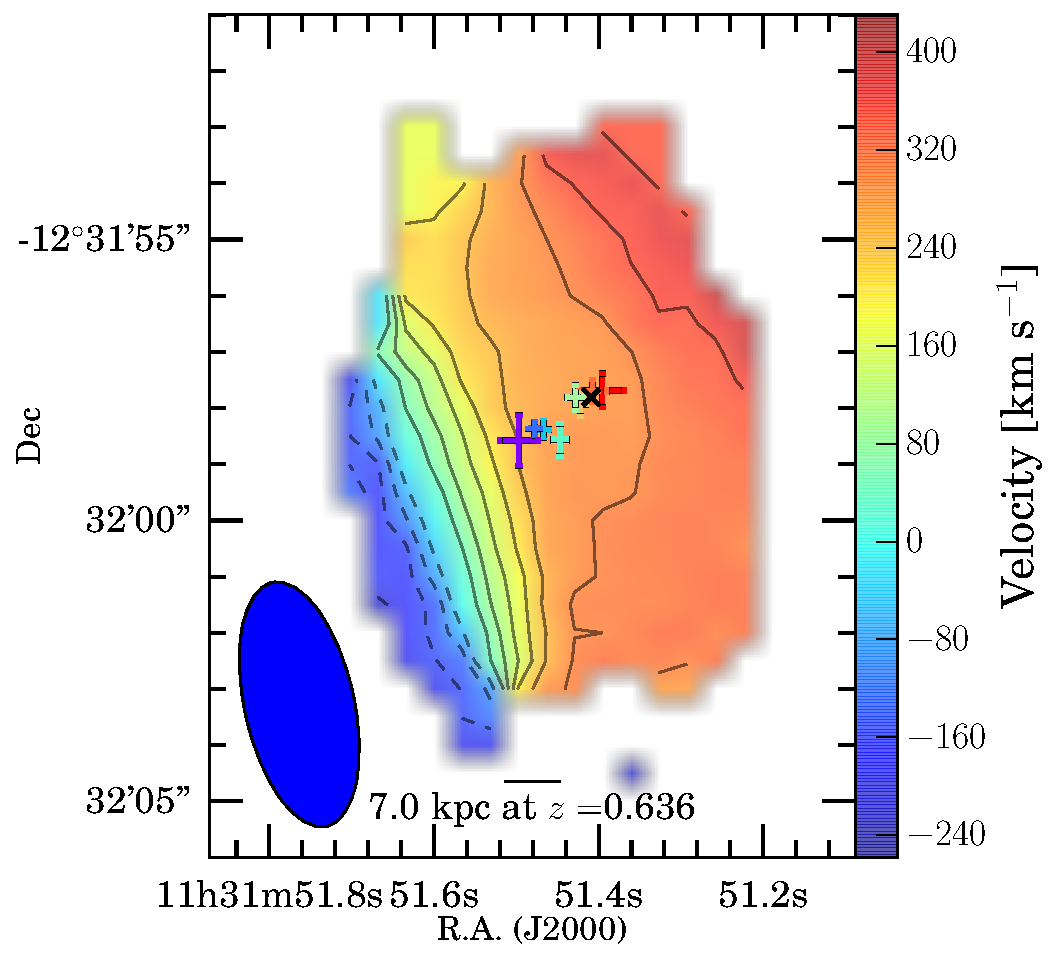
\includegraphics[trim= 0 0 0 0 clip, scale=0.43]{Figures/veloGradient_markers.pdf}
}
{
\caption{\fontsize{11pt}{12.5pt}\selectfont{\textbf{Image- and source-plane velocity gradient
of the \bco line emission in the AGN host galaxy RXJ1131.}
Source-plane positions reconstructed from the best-fit $uv$-plane lens modeling of 
our PdBI/NOEMA \bco data in the velocity-space
are indicated as color markers atop the observed first moment map. 
At the proposed resolution, we will be able to obtain a more accurate lens model, 
enabling us to resolve the intrinsic velocity gradient at finer details, and obtain a better-constrained rotation curve and dynamical mass estimate for this \interz quasar host galaxy.
}}
\label{fig:velo}}
\end{figure}

\begin{figure}[htbp]
\begin{center}
\includegraphics[trim=0 135 127 0, clip,width=1.0\textwidth]{Figures/combine3}
\caption{ \fontsize{11pt}{12.35pt}\selectfont{\textbf{Recent \bco data from
NOEMA (Leung et al., submitted).}}
{\em (a):}
Asymmetric double-horned line profile observed towards our target.
{\em (b):}
Spectra taken at three locations along the strongest velocity gradient,
demonstrating
differential lensing of the kinematic components of a gas-rich ``disc"
and the wealth of dynamical information that is already available at this resolution.
{\em (c):}
Observed spatial variations across different velocity components due to
differential lensing,
as shown by the red (redshifted),
green (line center), and blue (blueshifted) contours.
{\em (d):}
The observed velocity gradient is suggestive of a disc morphology at the current resolution limit.
The spectrally resolved lensed emission allows us to probe dynamical structures
on smaller spatial scales than otherwise possible.
{\em (e):}
An unusually high velocity gradient ($\gtrsim$400\,\kms) near the center of RXJ1131
may be a result of perturbations from the AGN, 
or internal turbulence due to interactions with the companion, 
or instability due to the huge gas reservoir. 
{\em (f):}
Channel maps of the CO emission (red)
overlaid on our best-fit lens models (grayscale).
The foreground lensing galaxy is represented by a black dot.
The reconstructed source morphology (magenta ellipses) is also suggestive of a
``disc".
{\em (g):}
Full resolution spectrum (yellow; same as panel $a$ but shown in log-scale) and the seven channels (dashed) used for lens modeling.
Using the magnification factors shown above the model channels, we recover an intrinsically symmetric profile (blue).
We here propose to observe \cco line in RXJ1131 at the spatial scales of \highz gas clumps
in order to investigate its molecular gas excitation, kinematical and dynamical state and examine how 
physical properties, e.g. stellar mass, dust temperature, SFR, morphology, clumpiness, internal gas dynamics, 
vary at intermediate redshift depending on the molecular gas conditions.
\label{fig:combine}}
\vspace{-2.15em}
\end{center}
\end{figure}

%%%%%%%%%%%%
\noindent \textbf{References}
{\fontsize{10pt}{12pt}\selectfont
	\bibliography{RXJ_SMA}
}


\end{document}
